\documentclass[12pt]{article}
\usepackage{indentfirst}
\usepackage{url}
\usepackage{pgf-pie}
\usepackage{graphicx}
\usepackage{enumitem}
\usepackage{tikz}
\usepackage{amsmath}

\newlength{\itemimagewidth}
\setlength{\itemimagewidth}{1.5cm}

\newlist{roadmap}{enumerate}{1}
\setlist[roadmap]{label={},leftmargin=*}

\newcommand{\roadmapitem}[3]{
  \item \begin{tikzpicture}[baseline={(0,-0.5)}]
    \node[anchor=west,inner sep=0pt,outer sep=0pt,minimum height=2em,minimum width=\itemimagewidth] (image) at (0,0) {\includegraphics[width=\itemimagewidth]{#1}};
    \node[anchor=west,inner xsep=5pt] at (image.east) {\parbox[t]{\dimexpr\linewidth-\itemimagewidth-5pt}{\textbf{#2}\par #3}};
  \end{tikzpicture}
}

\setlength{\oddsidemargin}{27mm}
\setlength{\evensidemargin}{27mm}
\setlength{\hoffset}{-1in}

\setlength{\topmargin}{27mm}
\setlength{\voffset}{-1in}
\setlength{\headheight}{0pt}
\setlength{\headsep}{0pt}

\setlength{\textheight}{235mm}
\setlength{\textwidth}{155mm}

\pagestyle{plain}

\renewcommand{\thefootnote}{\fnsymbol{footnote}}
\renewcommand{\labelitemi}{$\bullet$}

\begin{document}
\baselineskip 11pt


\begin{center}
  \textbf{\Large Swaptor Whitepaper} \\
  \vspace{1.5cc}

  { \sc Berry Block}\\
  \vspace{1.5cc}

  \begin{tabular}{c c c}
    \textsc{Marko Ivanković} & \textsc{Domagoj Ravlić} & \textsc{Hrvoje Kovačević} \\
    marko@berryblock.io      & domagoj@berryblock.io   & kova@berryblock.io        \\
  \end{tabular}
\end{center}
\vspace{1.5cc}

\begin{abstract}
  \noindent  Peer-to-peer (P2P) swaps on blockchain have the potential to greatly benefit users by eliminating the need for intermediaries in the exchange of assets. However, the use of P2P swaps on blockchain also presents several challenges, including trust issues that must be addressed in order to ensure their success.  Since there is no intermediary to oversee the exchange of assets, users must rely on the trustworthiness of the other party to the transaction. In the absence of a trusted third party, it is difficult to verify the authenticity and quality of the assets being exchanged, which can lead to disputes and losses for users.
  \\ \indent Furthermore, P2P swaps on blockchain are subject to potential security risks, such as hacking and fraud. Since the transactions are conducted directly between users, there is a greater risk of malicious actors attempting to exploit vulnerabilities in the system. This risk is exacerbated by the fact that blockchain transactions are irreversible, meaning that users have no recourse if their assets are stolen or lost.
  \\ \indent In this paper we describe Swaptor, a decentralized P2P exchange dapp which aims to eliminate problems mentioned above.

  \vspace{0.95cc}
\end{abstract}

\newpage

\tableofcontents

\newpage

\section{Motivation}

\subsection{Trust \& Security}
When conducting exchanges without intermediaries, users must depend entirely on the trustworthiness of the
other party involved often resulting in disputes and financial losses. Swaptor is a decentralized P2P exchange dapp designed to revolutionize
the way individuals swap assets with a mechanism to establish trust between parties, ensuring transparency
and reliability throughout the swap process. By leveraging blockchain technology and smart contracts,
Swaptor eliminates the need for intermediaries while prioritizing trust and security.

\subsection{Slippage problem}
With Swaptor's business model, users enjoy significant benefits compared to other platforms. By implementing
a fixed fee structure, Swaptor eliminates the common issue of slippage experienced on other platforms.
This means users can execute swaps with confidence, knowing that they will not incur unexpected losses due
to fluctuating prices during the transaction. Traditional platforms often charge a percentage of the transaction value,
which can eat into profits, therefore Swaptor's avoidance of percentage-based fees.

\subsection{Sustainable DAO}
The Swaptor project is driven by a vision to establish a sustainable DAO, a challenging endeavor in today's world.
Our DAO's strength lies in the fundamental and ongoing need for swapping. By harnessing the power of this simple action,
Swaptor's DAO aims to create a resilient backbone that benefits all participants. Through active participation in the
governance model, DAO members have the opportunity to earn a share of the fees, establishing a sustainable and rewarding ecosystem.

\newpage

\section{Architectural Overview} \label{form}
\indent As most modern dapps, Swaptor's architecture is a mix of on-chain and off-chain components:
\begin{itemize}
  \item \textbf{On-chain}: Smart contracts
  \item \textbf{Off-chain}: Backend, Frontend and Database
\end{itemize}

\subsection{On-chain Architecture}

\indent Smart contracts are written in Solidity, and their architecture is designed to be minimalistic.
Specifically, the Swaptor contract is a singular entity whose sole purpose is to verify digital signatures
and execute swaps upon successful verification. Digital signatures encode the specific terms under which a given swap is considered valid.

\subsubsection{Signatures}

In order to verify the signature, the smart contract must possess both the original swap elements
and the signature itself. Prior to being passed as an argument to one of the \textit{acceptSwap} functions,
these elements are encoded using the \textit{abi.encode} function. The signature is generated by creating a
\textit{keccak256} hash of the encoded arguments and signing it with the private key belonging to the user who creates the swap.
This method dramatically reduces the gas fees because the user never had to transfer their assets to Swaptor contract.

\subsubsection{Swap types}

At present, Swaptor facilitates the swapping of ERC-721 and ERC-20 tokens, enabling the execution of any combination of swaps involving these types of tokens.
In the future, Swaptor intends to extend its support to include native currency and ERC-1155 tokens.

\subsubsection{Fees}
To accept the swap, an address will need to pay a fixed fee of \$$5$ in the native currency, which is calculated using Chainlink oracles\cite{chainlink}. It should be noted that the fee is not fixed and may be subject to change.

\subsection{Off-chain Architecture}

\subsubsection{Backend}
The purpose of the backend is to reduce the number of operations on the blockchain,
which would result in higher gas fees paid by users. It also caches some information
retrieved from the blockchain to improve the user experience, such as reducing wait
times. Upon client request, it retrieves details about swaps, including the original
swap terms and signature.

\subsubsection{Frontend}
The Swaptor frontend application is a user interface that allows users to interact
with the Swaptor protocol on the supported networks. It enables users to easily swap
supported token types without the need for a centralized exchange. Each user is capable
of creating, deleting, sharing and accepting a swap. The application is accessible through a
web browser or mobile device and is designed to be user-friendly and intuitive.

\section{Swaptor token (SWPTR)}

Swaptor introduces its very own token called the Swaptor Token (SWPTR), which plays a
crucial role in the Swaptor governance model. By actively participating in voting rounds,
SWPTR holders have the opportunity to unlock a share of the rewards generated from Swaptor's swapping fees.
This mechanism allows for a fair and inclusive system that rewards only those who contribute to the platform's decision-making process.

\subsection{Governance}

\subsubsection{Initial stage}
As an essential part of the Swaptor governance model, the initial stage of the project will
involve the Swaptor developer team taking on the role of the Swaptor Committee. This dedicated
team will be responsible for facilitating the governance process by overseeing the submission of proposals,
managing the voting procedures, and ensuring the seamless operation of the Swaptor project.
The Swaptor Committee plays a crucial role in creating important questions and proposals that are later shared
with the Swaptor community for voting.

\subsubsection{Swaptor DAO}
Over time, the influence of the Swaptor developer team within the project will gradually diminish.
Initially, they will actively listen to the community's feedback and opinions through channels such as Twitter and Discord,
incorporating necessary code changes accordingly. Ultimately, the Swaptor project will evolve into a fully-fledged
decentralized autonomous organization (DAO). In this future state, any holder of the SWPTR token will have the
ability to propose changes to the project, and only those who possess SWPTR tokens will be eligible to participate
in the voting process. The voting power will be determined by the amount of SWPTR tokens held, as well as the proportionate
share of fees allocated as rewards for voters. After each vote, SWPTR holders will have the chance to unlock a portion of these rewards,
which promotes a fair and interactive ecosystem.


\begin{figure}[h]
  \centering
  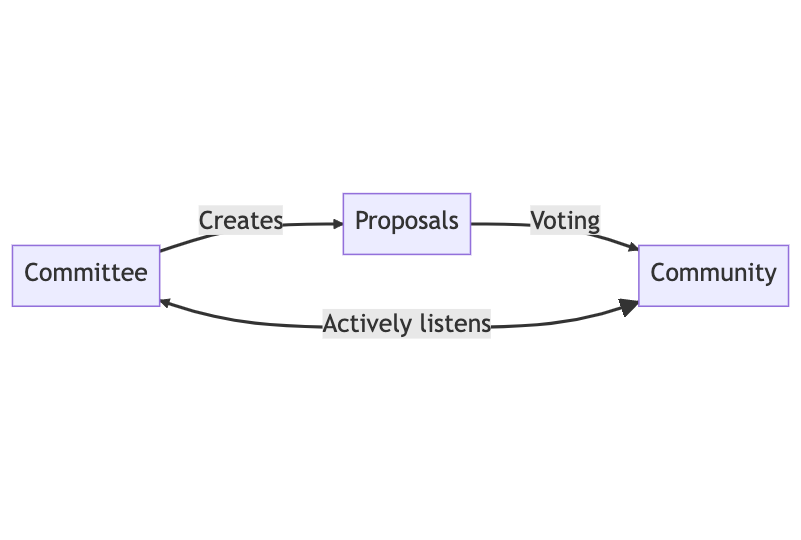
\includegraphics[width=18cm,height=8.8cm,keepaspectratio=true]{governance.png}
  \label{fig:docvsnur}
\end{figure}


\newpage

\subsection{Tokenomics}
The maximum supply of Swaptor tokens is set at 1,000,000. These tokens will be introduced in two distinct phases,
each serving a specific purpose in the evolution of the project.

\subsubsection{First phase}
In the first phase, which focuses on the initial stage of the project, the Swaptor developer team aims to involve
and empower contributors from the community. During this phase, a total of 300,000 tokens
(30\% of the total supply) will be made available for purchase.
The pricing of these tokens will be determined by the Swaptor developer team, ensuring a fair and reasonable value
that reflects the project's goals and potential.

\subsubsection{Second phase}
Moving to the second phase, the distribution of the remaining 700,000 tokens
(70\% of the total supply) takes a different approach. Rather than being sold or offered directly,
tokens will be minted exclusively through successful swaps conducted via the Swaptor smart contract.
With each successful swap, where users exchange one cryptocurrency for another using Swaptor,
one token will be allocated to each of the participant. This mechanism promotes active engagement with the platform
and incentivizes users to participate in swaps, contributing to the growth and liquidity of the Swaptor ecosystem.
It is important to mention that every token that is not sold in the first phase will be minted during this phase.

\vspace{1.5cc}
By adopting this two-phase approach, Swaptor aims to involve early contributors while also fostering
a dynamic and sustainable token distribution model. It ensures that tokens are not only accessible to
those who support the project from its inception but also rewards users who actively participate in successful swaps,
aligning incentives and creating a vibrant community of token holders.

\vspace{2cc}

\begin{figure}[h]
  \centering
  \begin{tikzpicture}
    \pie[text=inside]{30/Public sale, 70/Protocol minting}
  \end{tikzpicture}
  \caption{Token distribution}
  \label{fig:pie-chart}
\end{figure}


\newpage

\section{Roadmap}

\begin{roadmap}
  \roadmapitem{swaptor.png}{Q3 2023}{
    Deployment of Swaptor contracts to Ethereum mainnet
  }

  \roadmapitem{swaptor.png}{Q4 2023}{
    Multichain \& ENS names support
  }

  \roadmapitem{swaptor.png}{Q1 2024}{
    Support for remaining token standards
  }

  \roadmapitem{swaptor.png}{Q2 2024}{
    Mobile app development
  }

  \roadmapitem{swaptor.png}{Q3 2024}{
    Swaptor messaging \& notification system - enabling direct communication
    between users through Swaptor website
  }

  \roadmapitem{swaptor.png}{Q4 2024 - Q1 2025}{
    Order book model for ERC-20 tokens.
  }
\end{roadmap}

\begin{thebibliography}{9}
  \bibitem{chainlink} What is an oracle in blockchain? explained | chainlink, \url{https://chain.link/education/blockchain-oracles}
\end{thebibliography}

\end{document}